% !TeX spellcheck = fr_FR
\documentclass[../main.tex]{subfiles}

\begin{document}
	
Les réseaux de neurones sont implémentés en utilisant la librairie \textsf{PyTorch} \cite{paszke2017automatic}, permettant de faire du calcul tensoriel avec différentiation automatique (pour calculer les gradients).\footnote{Le code est ici: \url{https://github.com/ManifoldFR/point-process-nets}} L'entraînement utilise l'algorithme de descente du gradient Adam \autocite{AdamKingmaB14}.

Une fonctionnelle de perte possible, utilisée dans \autocite{meiEisnerNeuralHawkes} pour entraîner le réseau sur des données réelles, est la log-vraisemblance \eqref{eq:likelihood} d'une suite d'événements $\{(t_i,k_i)\}_i$. La formule\footnotemark~suivante est démontrée \cite[15]{meiEisnerNeuralHawkes}: 
\begin{equation}\label{eq:explicitLikelihood}
\mathcal{L}\left(\{(t_i,k_i)\}_i\right)
=
\sum_{i:\, t_i < T} \log\lambda^{k_i}_{t_i} - \int_0^T \bar\lambda_t\,dt
\end{equation}
où on a noté $\mathbf{1} = {(1,\ldots,1)}^\intercal\in\RR^K$. Le second terme est une intégrale. Elle peut être estimée par une méthode de Monte Carlo, comme le suggèrent \citeauthor{meiEisnerNeuralHawkes}. Plus de détails sur l'estimateur utilisé sont donnés dans l'annexe \ref{ssec:likelihoodComputation}.

\footnotetext{Il faut noter ici que dans cette expression $\lambda_{t_i}^{k_i}$ est la valeur de l'intensité à l'instant $t_i$, juste avant l'événement $(t_i, k_i)$.}

On peut générer des séquences d'événements à partir des réseaux de neurones en utilisant l'algorithme de \textit{thinning} d'\citeauthor{ogata1981} \autocite{ogata1981} avec les modifications nécessaires pour l'étape de rejet (voir annexe \ref{ssec:thinning}).

Pour la prédiction d'événement, on évalue le réseau sur un début de séquence $\{(t_j,k_j)\}_{j < i}$, permettant d'obtenir l'historique du processus jusqu'à $\mathcal{F}_{t_{i-1}}$. Le meilleur estimateur au sens $L_2$ de $t_i$ avec l'information $\mathcal{F}_{t_{i-1}}$ est
\[
	\hat{t}_i = \EE\left[ t_i \mid \mathcal{F}_{t_{i-1}} \right]
\]
\citeauthor{meiEisnerNeuralHawkes} suggèrent une méthode pour évaluer cette espérance. En effet, la loi du temps d'attente avant le prochain événement conditionnellement à $\mathcal{F}_{t_{i-1}}$ s'exprime par la densité de probabilité:
\begin{equation}\label{eq:nextIncrementDensity}
	p_i(t-t_{i-1}) = \bar\lambda_t\exp\left(-\int_{t_{i-1}}^t\bar\lambda_u\,du\right)
\end{equation}
et on a l'expression de l'estimateur:
\begin{equation}\label{eq:nextEventTimeEstimator}
	\hat{t}_i = t_{i-1} + \int_0^\infty u p_i(u)\,du.
\end{equation}
Pour le type $k_i$, on utilise l'estimateur
\begin{equation}
\hat{k}_i = \argmax_{k} \EE\left[\frac{\lambda^{k}_{t_i}}{\bar\lambda_{t_i}}\middle| \mathcal{F}_{t_{i-1}} \right] = \argmax_k \int_0^\infty \frac{\lambda^{k_i}_{t_{i-1}+u}}{\bar\lambda_{t_{i-1}+u}} p_i(u)\,du.
\end{equation}

La \autoref{fig:probDensityPlot2DLSTM} illustre cette densité de probabilité et le choix de l'estimation $\hat{t}_i$ dans le cas du modèle LSTM avec $K=2$.

\begin{figure}[!ht]
	\centering
	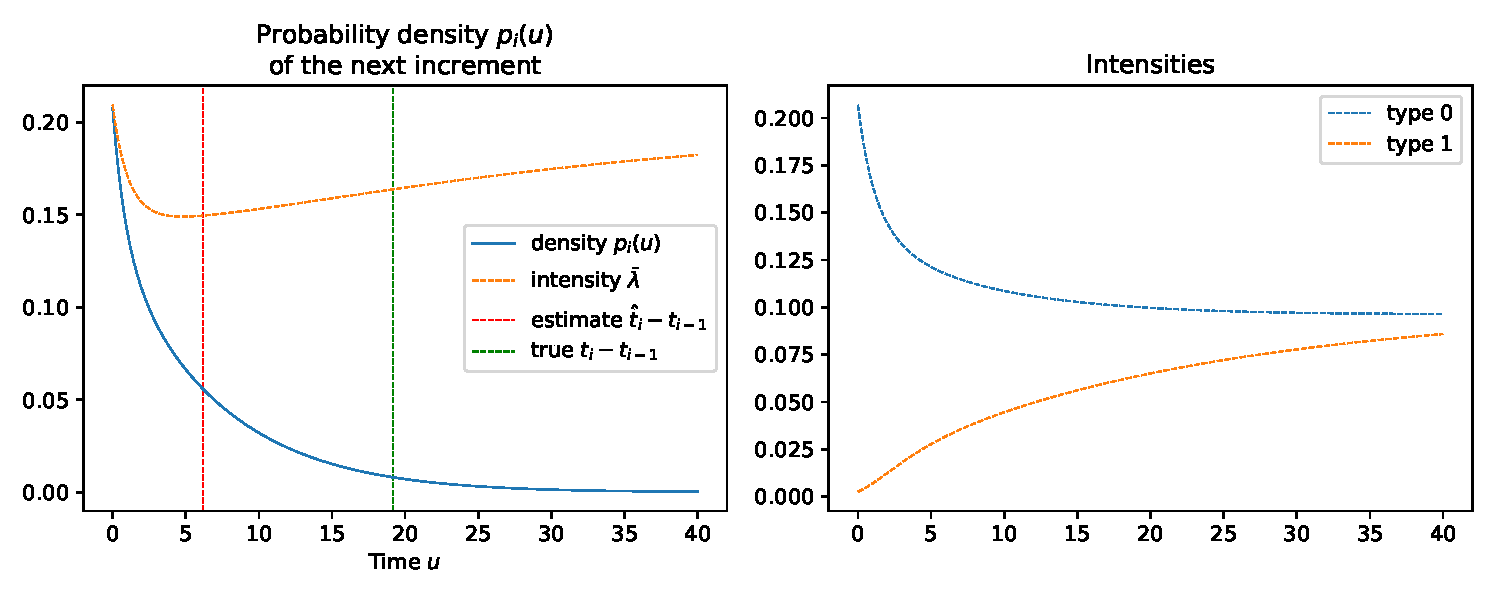
\includegraphics[width=\linewidth]{../notebooks/lstm_2d_prediction_graphs.pdf}
	\caption{Densité de probabilité du prochain événement, pour la prédiction du prochain événement sur des données Hawkes 2D avec le LSTM.}\label{fig:probDensityPlot2DLSTM}
\end{figure}

Pour le réseau récurrent RMTPP, le modèle s'entraîne sur la fonction perte
\begin{equation}
l =  \sum_i(\log\mathcal{P}(k_{i+1} | \mathcal{F}_{t_{i-1}}) + \log f(t_{i+1}|  \mathcal{F}_{t_{i-1}}   )  )
\end{equation}
qui est ensuite sommée sur l'ensemble des séquences de l'ensemble d'entraînement.

\end{document}